\documentclass[conference]{IEEEtran}
\IEEEoverridecommandlockouts
% The preceding line is only needed to identify funding in the first footnote. If that is unneeded, please comment it out.
\usepackage{cite}
\usepackage{amsmath,amssymb,amsfonts}
\usepackage{algorithmic}
\usepackage{graphicx}
\graphicspath{ {./images/} }
\usepackage{textcomp}
\usepackage{xcolor}
\def\BibTeX{{\rm B\kern-.05em{\sc i\kern-.025em b}\kern-.08em
    T\kern-.1667em\lower.7ex\hbox{E}\kern-.125emX}}
\begin{document}

\title{Acoustic Crack Detection on Material Coupons Using a Deep Convolutional Neural Network
}

\author{\IEEEauthorblockN{1\textsuperscript{st} Sarah Malik}
\IEEEauthorblockA{\textit{dept. name of organization (of Aff.)} \\
\textit{name of organization (of Aff.)}\\
City, Country \\
email address or ORCID}
\and
\IEEEauthorblockN{2\textsuperscript{nd} Michael Shenoda}
\IEEEauthorblockA{\textit{dept. name of organization (of Aff.)} \\
\textit{name of organization (of Aff.)}\\
City, Country \\
email address or ORCID}
\and
\IEEEauthorblockN{3\textsuperscript{rd} Jeremy Fernsler}
\IEEEauthorblockA{\textit{Computer Science} \\
\textit{Drexel University}\\
Glendale, CA, USA \\
jfernsler@drexel.edu}
\and
}

\maketitle

\begin{abstract}
We present a method for detecting structural cracks in a material using acoustic
data analyzed by a convolutional neural network (CNN). Material fatigue leading
to cracks and faults is a serious problem in vehicles, infrastructure, and many
other sectors of engineering. Work has already been done to analyze the passive
signals from MEMs piezo sensors fixed to a surface (CITATION). Our method takes
the captured waveform from a material sample under load, converts the waveform
into frequency space and passes it through a classifying CNN to detect
whether or not the sample contains a crack. We demonstrate the accuracy of such
a system and assess the viability of a CNN for acoustic crack detection.
\end{abstract}

\section{Introduction}

Short history of prior work related to this from sarah

\section{Data}

\subsection{Data Origin and Pre-Processing}

Our data comes from a laboratory test where a coupon of material is placed under
increasing tension until it delaminates, develops a crack, and fails. MEMs piezo
sensors are bonded to the coupon prior to the test and the output is recorded at
a sampling rate of 5Mhz. This results in individual waveforms saved in plain text
files consisting of just over 6000 samples each up to and after the crack as
developed. The load value is recorded simultaneously and a severe drop in load
value can be marked as a fully developed crack appearing. The time at which this
drop occurs is recorded and we can use this to label our data as un-cracked
(pre-drop) or cracked (post-drop).

For our purposes, we need to collect the data and do a minimal amount of
pre-processing. We had access to over 30,000 individual waveform files collected
over two tests. From prior work [citation] one channel was chosen from each
test as the best candidate. Each file is read in, and relevant data is stripped from the
headers such as time, which sensor channel is being read, and the sequential
number of each waveform as it was collected. The data was stored in a Pandas
dataframe and the crack time (determined by the aforementioned method) was used
to label each waveform. A column was created to hold the entropy value for
each waveform as this was the measurement used within the lab to attempt to
identify when a crack moment happened. We were unsure if this would be useful
in our model, so we stored it along side our waveform data if needed. The
waveforms often contained long stretches of zero values where the tension machine
was not applying force and thus creating no new data from the sensor. A new column
was created in the dataframe which contained the waveform with stripped zeros.
This dataframe is pickled for storage and quick reads for training. After selecting
proper samples and labeling it, we had 1665 total crack samples and several thousand
non-crack samples. We shuffled all non-crack samples and selected a matching 1665
at random for a total training set of 3330 labeled waveforms, each containing at
least 3000 wave samples for each observation.

\subsection{Data Within the Model}

The no-zero waveforms are read in and an evenly distributed 80/20 split is generated
for training and validation purposes. We created an WaveformInputLayer which
takes a waveform and casts it to frequency space as a Mel Spectrogram using a
Short Time Fast Fourier Transform (STFFT). The window of time used by the STFFT
constrains the number of frequencies that can be analyzed. We use this as a tunable
hyperparameter (N). Adjusting the value of N changes the width and height of the Mel
Spectrogram so we constrain the size of this by resizing it using either nearest
neighbor or bilinear filtering - another hyperparameter choice, along with the
final size of the image. These 2D matrices are stored as a tensor and passed into
the rest of the CNN.


\section{Model Methodolgy}

Approach to the CNN

Custom Layers

Etc...

\subsection{Hyperparameters and Tuning}\label{AA}

Tunable parameters

How we found them

\section{Results and Discussion}

Charts and tables

\begin{table}[htbp]
\caption{Table Type Styles}
\begin{center}
\begin{tabular}{|c|c|c|c|}
\hline
\textbf{Table}&\multicolumn{3}{|c|}{\textbf{Table Column Head}} \\
\cline{2-4} 
\textbf{Head} & \textbf{\textit{Table column subhead}}& \textbf{\textit{Subhead}}& \textbf{\textit{Subhead}} \\
\hline
copy& More table copy$^{\mathrm{a}}$& &  \\
\hline
\multicolumn{4}{l}{$^{\mathrm{a}}$Sample of a Table footnote.}
\end{tabular}
\label{tab1}
\end{center}
\end{table}

\begin{figure}[htbp]
\centerline{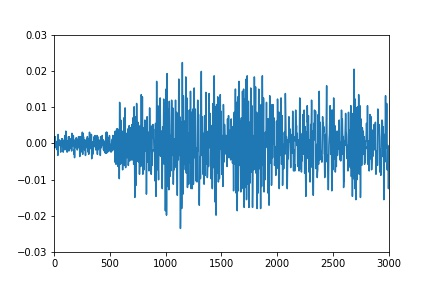
\includegraphics[width=.5\textwidth]{waveform_0.jpg}}
\caption{Mel Spectrogram.}
\label{fig}
\end{figure}

\begin{figure}[htbp]
\centerline{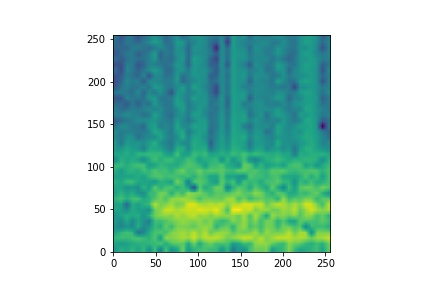
\includegraphics[width=.5\textwidth]{spectrogram_0.jpg}}
\caption{Mel Spectrogram.}
\label{fig}
\end{figure}





\section{Conclusion}

Did it work?

\section*{References}

Stand in only:

Please number citations consecutively within brackets \cite{b1}. The 
sentence punctuation follows the bracket \cite{b2}. Refer simply to the reference 
number, as in \cite{b3}---do not use ``Ref. \cite{b3}'' or ``reference \cite{b3}'' except at 
the beginning of a sentence: ``Reference \cite{b3} was the first $\ldots$''

Number footnotes separately in superscripts. Place the actual footnote at 
the bottom of the column in which it was cited. Do not put footnotes in the 
abstract or reference list. Use letters for table footnotes.

Unless there are six authors or more give all authors' names; do not use 
``et al.''. Papers that have not been published, even if they have been 
submitted for publication, should be cited as ``unpublished'' \cite{b4}. Papers 
that have been accepted for publication should be cited as ``in press'' \cite{b5}. 
Capitalize only the first word in a paper title, except for proper nouns and 
element symbols.

For papers published in translation journals, please give the English 
citation first, followed by the original foreign-language citation \cite{b6}.

\begin{thebibliography}{00}
\bibitem{b1} G. Eason, B. Noble, and I. N. Sneddon, ``On certain integrals of Lipschitz-Hankel type involving products of Bessel functions,'' Phil. Trans. Roy. Soc. London, vol. A247, pp. 529--551, April 1955.
\bibitem{b2} J. Clerk Maxwell, A Treatise on Electricity and Magnetism, 3rd ed., vol. 2. Oxford: Clarendon, 1892, pp.68--73.
\bibitem{b3} I. S. Jacobs and C. P. Bean, ``Fine particles, thin films and exchange anisotropy,'' in Magnetism, vol. III, G. T. Rado and H. Suhl, Eds. New York: Academic, 1963, pp. 271--350.
\bibitem{b4} K. Elissa, ``Title of paper if known,'' unpublished.
\bibitem{b5} R. Nicole, ``Title of paper with only first word capitalized,'' J. Name Stand. Abbrev., in press.
\bibitem{b6} Y. Yorozu, M. Hirano, K. Oka, and Y. Tagawa, ``Electron spectroscopy studies on magneto-optical media and plastic substrate interface,'' IEEE Transl. J. Magn. Japan, vol. 2, pp. 740--741, August 1987 [Digests 9th Annual Conf. Magnetics Japan, p. 301, 1982].
\bibitem{b7} M. Young, The Technical Writer's Handbook. Mill Valley, CA: University Science, 1989.
\end{thebibliography}
\vspace{12pt}



\end{document}
